\documentclass[12pt]{article}

\usepackage[utf8]{inputenc}
\usepackage[T1]{fontenc}
\usepackage[french]{babel}
\usepackage{hyperref}
\usepackage{graphicx}
\usepackage{listings}
\usepackage[linesnumbered,ruled,french,onelanguage]{algorithm2e}
\lstset{numbers=left, numberstyle=\tiny, stepnumber=1, numbersep=6pt}
\makeatletter 
\g@addto@macro{\@algocf@init}{\SetKwInput{KwOut}{Sortie}}
\makeatother
\title{Aide à la Décision - Othello}
\author{Antonin Boyon \and Quentin Legot \and Arthur Page}
\date{\today}

\begin{document}

\maketitle
\thispagestyle{empty}
\setcounter{page}{0}
\newpage

\tableofcontents
\newpage

\section{Introduction}

Le but de notre projet était de concevoir un algorithme de recherche performant sur un jeu d' \textit{Othello}. Le jeu est le plus abstrait possible, la partie nous intéressant étant la réalisation d'un algorithme de recherche efficace. Il est ainsi impossible de jouer au jeu, on ne peut que regarder le résultat d'une partie entre deux joueurs artificiels.\\
Une fois le jeu et l'algorithme de recherche implémentés, nous serons en mesure d'analyser ce dernier pour définir ses paramètres de fonctionnement optimaux. Nous aborderons dans un premier temps l'implémentation du jeu, puis celle de l'algorithme et enfin la présentation et l'analyse des mesures observées.


\section{Organisation du code}
Notre code se compose de plusieurs classes dont nous allons détailler les rôles ci-dessous. 
\begin{itemize}
\item La classe STATE: \\ Cette classe représente un état du jeu à un moment donné avec différents paramètres comme le nombre de pions de chaque joueur et leur position sur un plateau de jeu. Elle possède plusieurs méthodes lui permettant de créer une copie d'elle-même, de s'afficher, de trouver les coups possibles pour un joueur ou encore de jouer un coup.
\item La classe PAIR: \\ Cette classe nous a permis de représenter les coups possibles par une paire pion de départ, pion d'arrivée.
\item Les classes PLAYER: \\ Elles permettent de simuler un joueur, il en existe 4, la classe mère PLAYER et les classes filles NEGAMAXPLAYER, RANDOMPLAYER et ALPHABETAPLAYER. La classe RANDOMPLAYER renvoie un coup au hasard parmi les coups possibles. Pour le fonctionnement des deux autres classes, il est détaillé dans les pages qui suivent.
\item La classe POINT: \\ Elle nous permet simplement de représenter un point du plateau de jeu avec une coordonnée X et une coordonnée Y.
\end{itemize}
\section{L'algorithme de recherche}
\subsection{Algorithme de base}

Nous avons utilisé un algorithme Negamax pour résoudre le problème, représenté en pseudo-code ci-dessous.

\lstinputlisting[language=Java]{NegamaxPlayer.java}

\newpage
\subsection{Algorithme d'élagage}

Afin d'améliorer les performances de notre algorithme de base, nous avons implémenté une version avec élagage Alpha-Beta, plus performante.

\lstinputlisting[language=Java]{AlphaBetaPlayer.java}

\newpage
\section{Mesures}

\subsection{Présentation}

Les graphiques qui vont suivre ont été conçus à l’aide des algorithmes AlphaBeta et Negamax.\\
Ils sont l’objet de comparaisons entre les algorithmes, en fonction de leur type ou du joueur concerné (premier ou second joueur).\\
Ils traduisent la complexité de l’algorithmes (le nombre de nœuds traversés) au fur et à mesure des tours de la partie.\\
Le premier joueur est associé à la courbe rouge et le deuxième à la bleue.\\
La profondeur de recherche des deux joueurs sera toujours la même.\\

Tout les tests incluant un temps ont été fait sur la même machine et en même temps: Raspberry pi 3 avec un processeur Quad Core 1.2GHz 64bit sous Raspbian OS 32 bits sans Bureau.
\newpage
\subsection{AlphaBeta}

\subsubsection{Profondeur 1}

\begin{figure}[!h]
   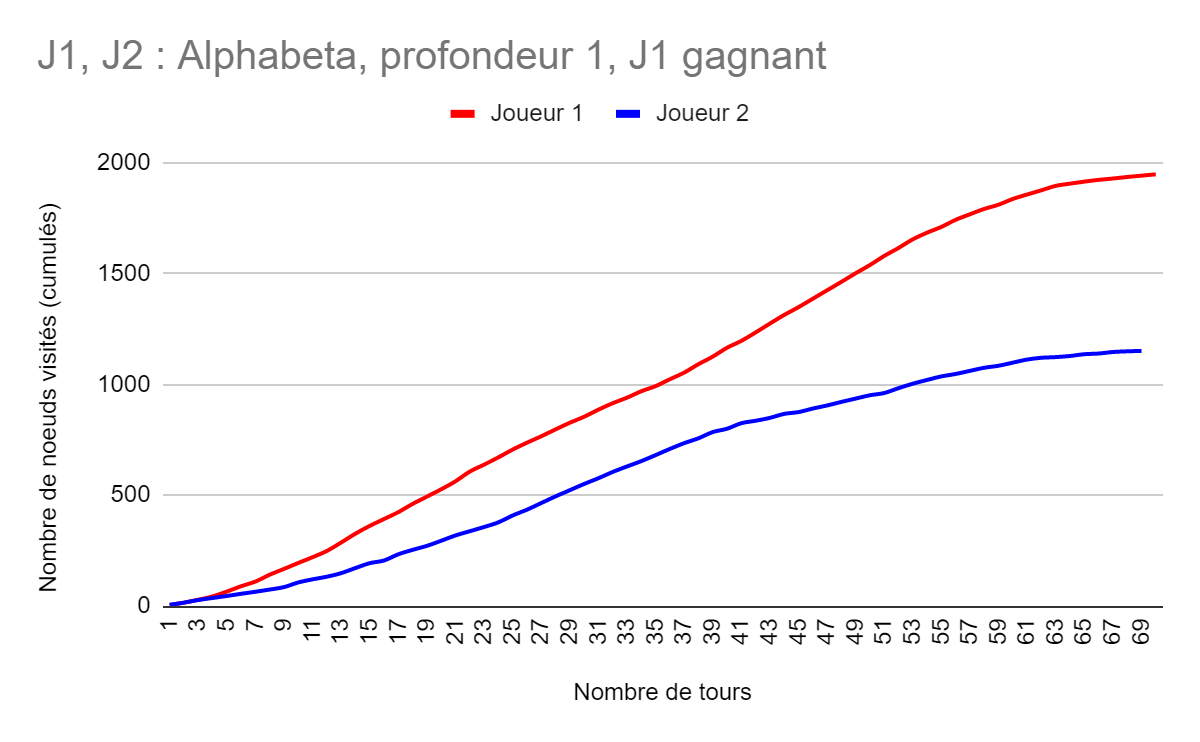
\includegraphics[width=\textwidth]{prof1alphabeta.png}
\end{figure}

Le joueur 1 obtient assez vite (tour 5) un avantage (il possède plus de possibilités) qui augmente au fur et à mesure des tours. A son maximum (fin de la partie) cet avantage est 69\% plus important par rapport au second joueur.\\
L’augmentation de la complexité est plutôt linéaire.\\
Il semblerait que jouer en premier est un avantage.
\newpage
\subsubsection{Profondeur 2}

\begin{figure}[!h]
   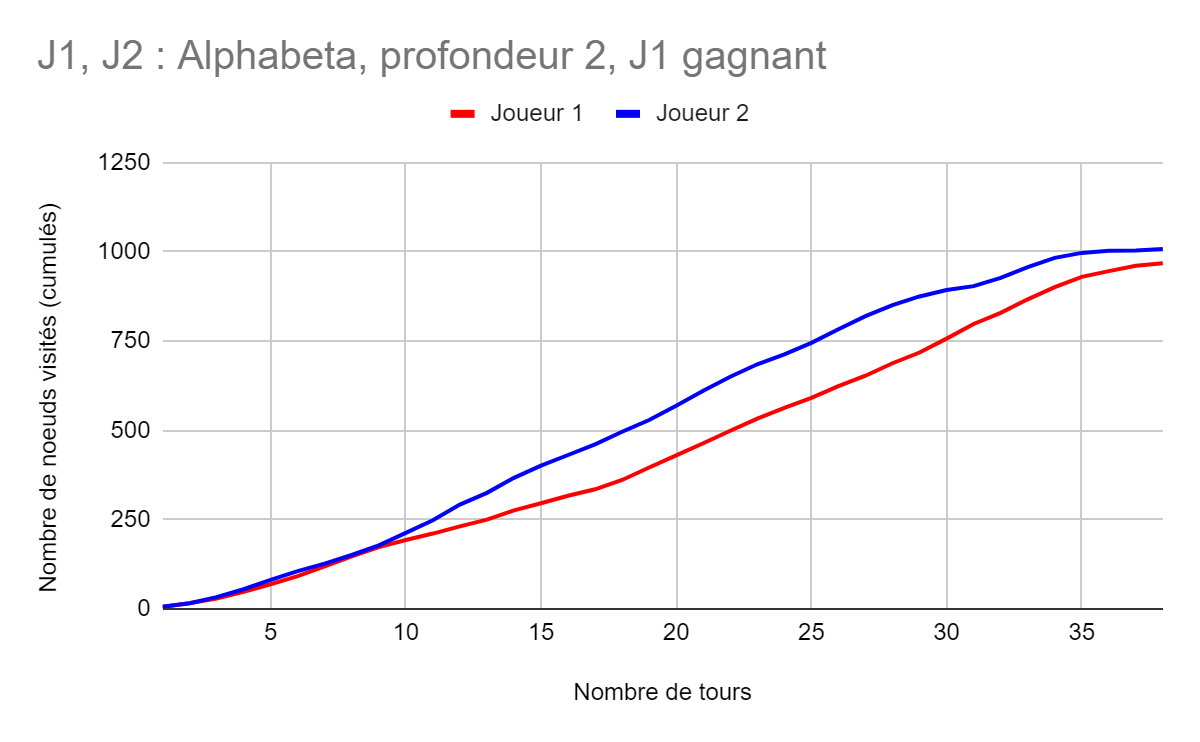
\includegraphics[width=\textwidth]{prof2alphabeta.png}
\end{figure}

Malgré qu’il soit second à jouer, joueur 2 obtient un avantage au niveau du tour 10 environ. Cet avantage augmente jusqu’au tour 30, avec un pic à 30\% par rapport au joueur 1, mais reste marginal. Il se réduit ensuite jusqu’à la fin de la partie.\\
Le nombre de tour est largement inférieur par rapport au précédent graphique. La complexité du joueur 1 est deux fois moins importante que sur le graphique précédent, malgré la profondeur plus importante.\\
Mais malgré cet avantage, la victoire est pour le joueur 1.\\
La courbe est linéaire, comme sur la graphique précédent.\\
Être le premier à jouer semble donner un avantage, et le nombre de possibilités du joueur 2 plus important n’était pas suffisant pour le résorber. La profondeur ne semble pas forcément augmenter le nombre de possibilités.
\newpage
\subsubsection{Profondeur 3}

\begin{figure}[!h]
   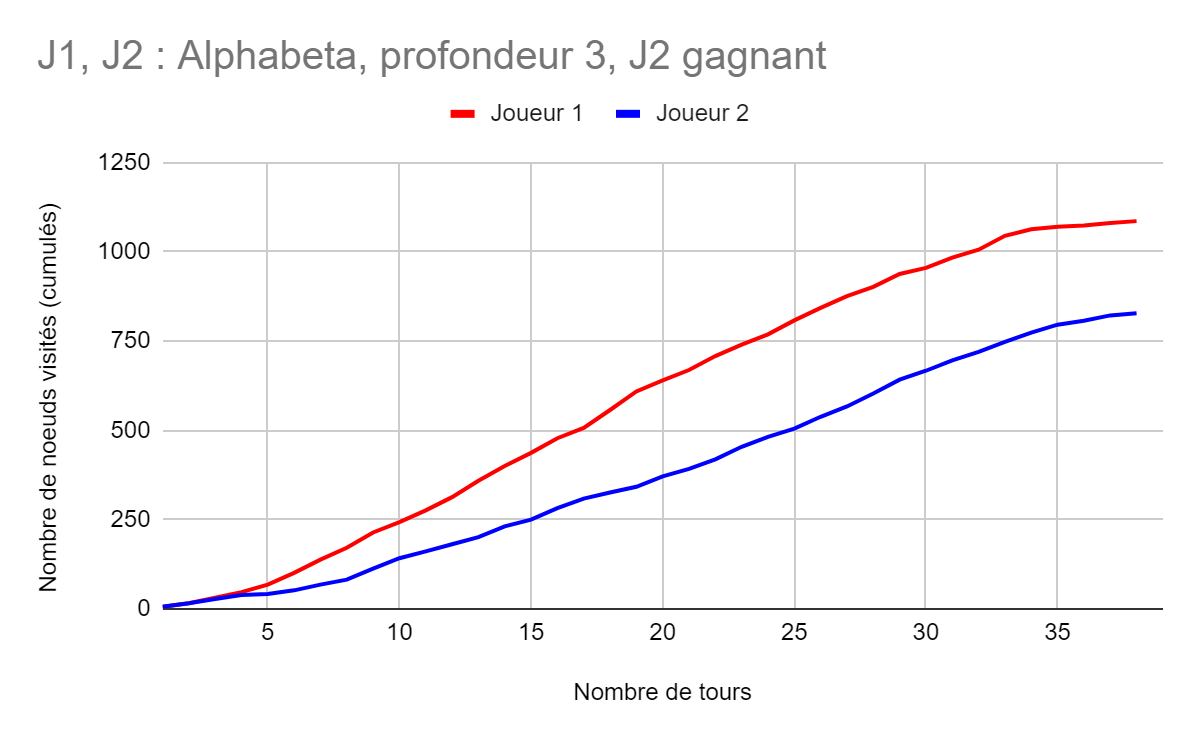
\includegraphics[width=\textwidth]{prof3alphabeta.png}
\end{figure}

Comme pour la profondeur 1, le joueur 1 a tôt, au tour 5 environ, un avantage qui augmente également au fur et à mesure de la partie et gagne cette dernière.\\
La situation est similaire à AlphaBeta de profondeur 1.
\newpage
\subsubsection{Profondeur 4}

\begin{figure}[!h]
   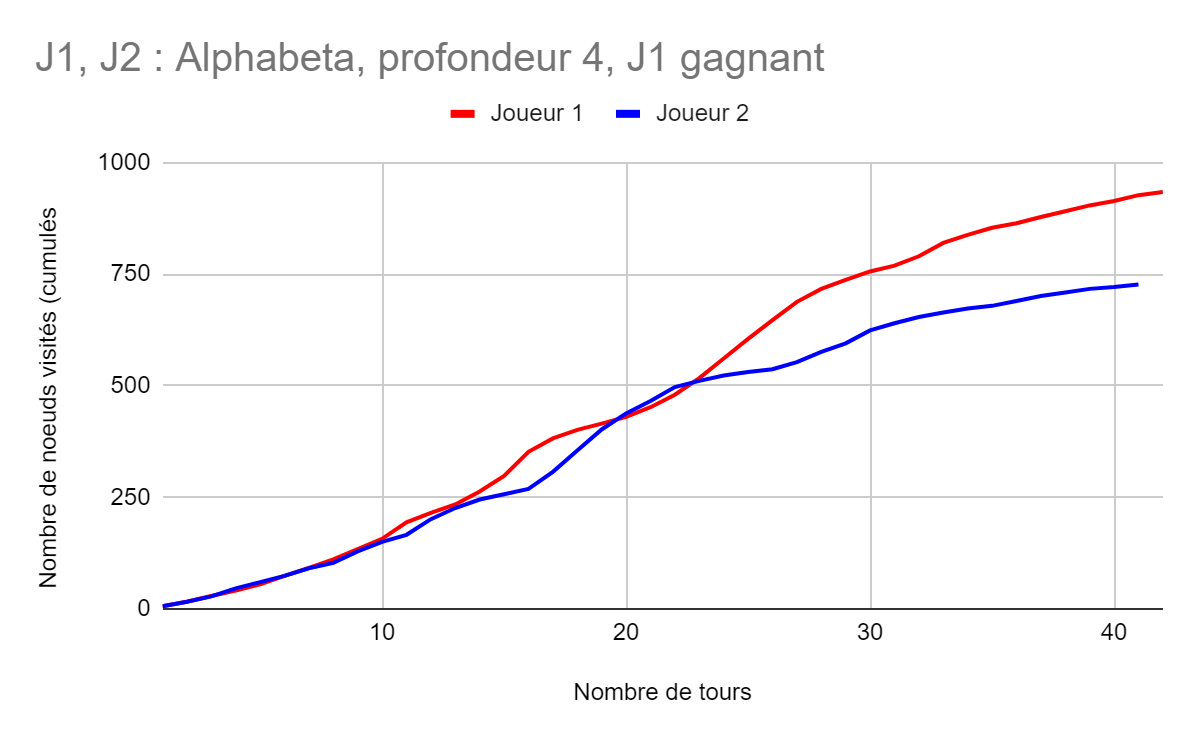
\includegraphics[width=\textwidth]{prof4alphabeta.png}
\end{figure}

Similaire au graphique de profondeur 2, le second joueur possède un avantage à partir du tour 5 environ. Mais au tour 20 cet avantage augmente drastiquement pour atteindre 100\% de plus, en fin de partie, par rapport au joueur 1. La complexité du premier joueur est particulièrement basse, presque 70\% moins importante qu’avec la profondeur de 1.\\
Pour la première fois, c’est le second joueur qui gagne la partie.\\
L’avantage très important du joueur 2 lui a permis de l’emporter, malgré son désavantage de joueur en second.\\

\begin{figure}[!h]
   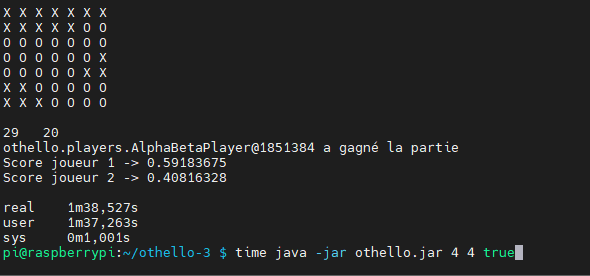
\includegraphics[width=\textwidth]{prof4alphabeta-console.png}
\end{figure}

Le temps de résolution de cet algorithme est de 1 minute et 12 secondes pour un total de 2 226 nœuds visités (pour les deux joueurs).

\subsubsection{Profondeur 5}

\begin{figure}[!h]
   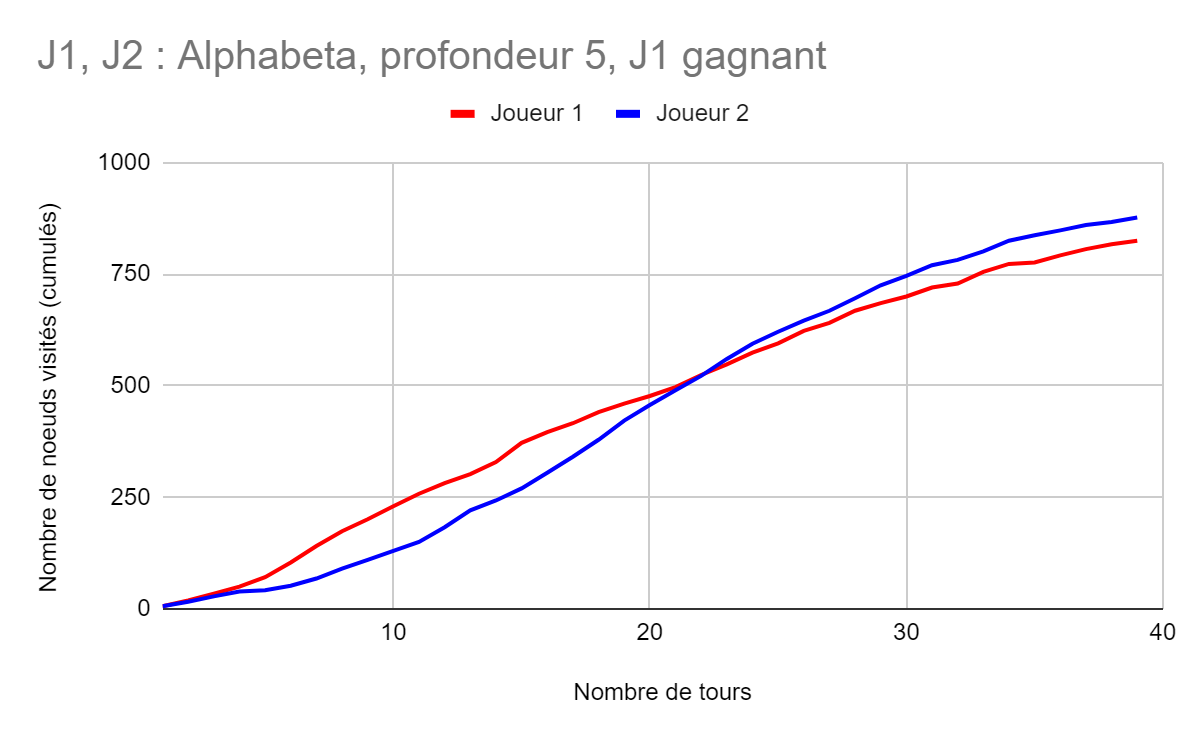
\includegraphics[width=\textwidth]{prof5alphabeta.png}
\end{figure}

Au tour 5 environ, le premier joueur obtient un léger avantage qui se résorbent au tour 30.\\
Pour le reste de la partie, il n’y a pas de réelle avantage d’un joueur.\\
Conformément aux observations précédentes, sans avantage du joueur 2, c’est le premier joueur qui l’emporte.

\begin{figure}[!h]
   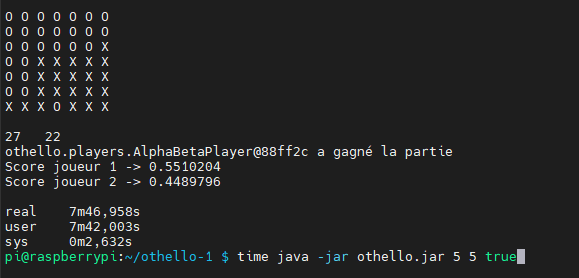
\includegraphics[width=\textwidth]{prof5alphabeta-console.png}
\end{figure}

Pour 3 094 nœuds visités, l’algorithme dure 6 minutes et 54 secondes. 

\subsubsection{Conclusion d’Alphabeta}

Jouer en premier donne un avantage. Il faut au second joueur un avantage conséquent (situé entre 30\% et 100\% par rapport au premier) pour lui permettre de l’emporter.\\
De plus, c’est sur les profondeur pairs que le second joueur semble posséder un avantage.\\
L’augmentation de la profondeur de l’algorithme AlphaBeta n’augmente pas forcément la complexité de ce dernier. Cependant l’augmentation de la complexité en fonction du nombre de tour est relativement linéaire.\\
Le temps de résolution des algorithme pour des petites profondeurs (1, 2, 3) est de quelques secondes mais augmente drastiquement avec la profondeur, AlphaBeta(5) s’exécute pendant plusieurs minutes. 

\subsection{Negamax}

\subsubsection{Profondeur 1}

\begin{figure}[!h]
   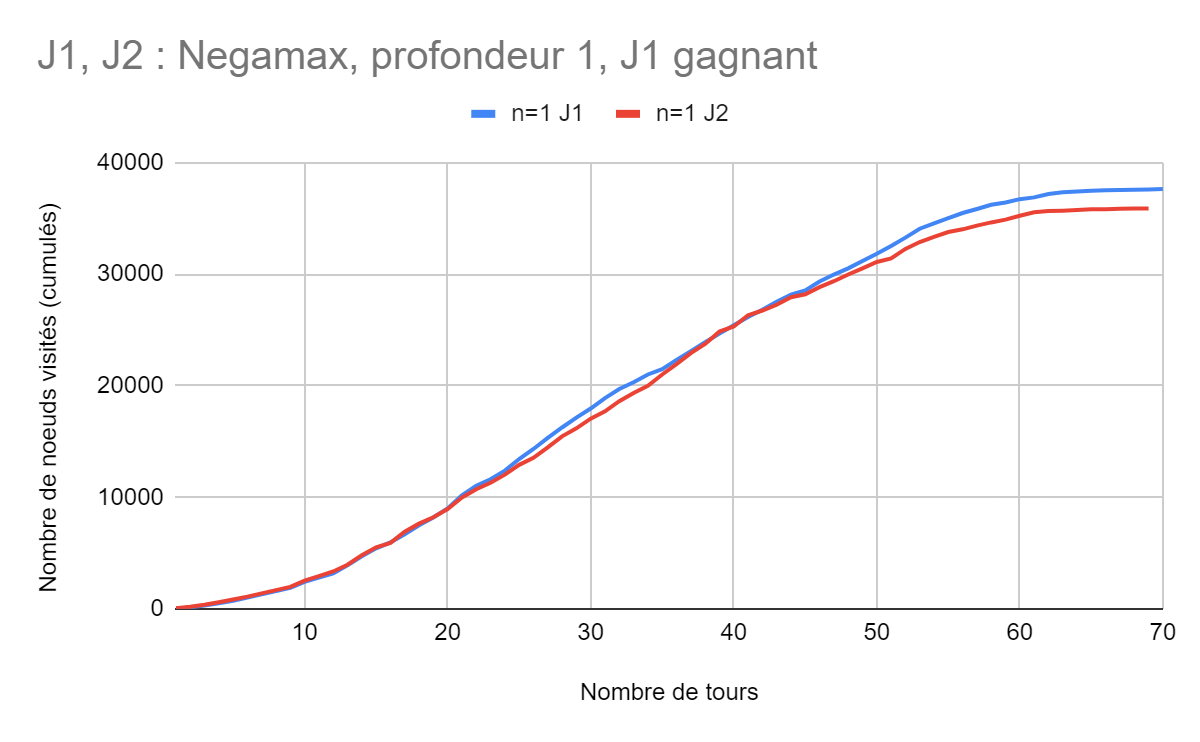
\includegraphics[width=\textwidth]{prof1negamax.png}
\end{figure}

Aucun des joueurs n’a d’avantage particulier.\\
La complexité est environ 20 fois plus importante qu’AlphaBeta.\\
Le joueur 1 est le gagnant. Avec cet algorithme aussi il semblerait que le premier joueur possède un avantage.\\
L’augmentation de la complexité est moins importante au début et à la fin de partie mais est assez linéaire.

\subsubsection{Profondeur 2}

\begin{figure}[!h]
   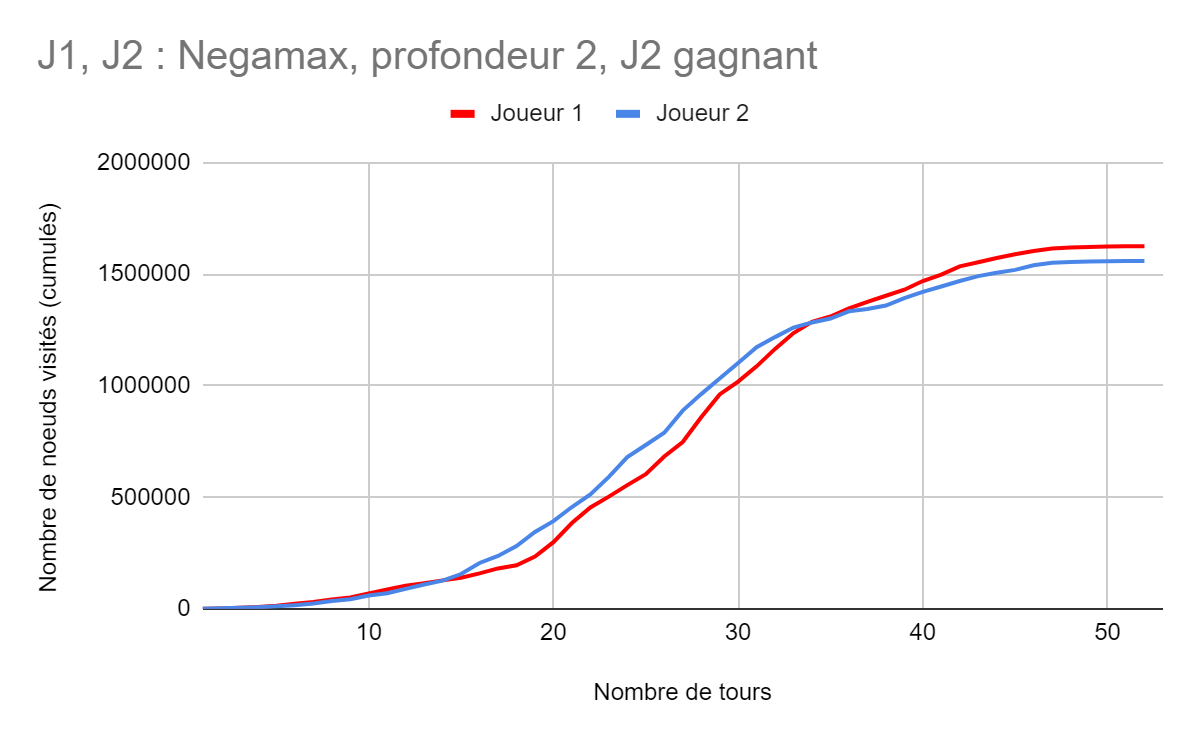
\includegraphics[width=\textwidth]{prof2negamax.png}
\end{figure}

La complexité est 40 fois plus importante qu’avec la profondeur précédente.\\
La forme de la courbe est similaire au graphique précédent.\\
Aucun joueur n’a d’avantage majeur au cours de la partie. Le second joueur a un petit avantage qui commence au tour 15 et qui finit au tour 33 où le premier prend l’avantage, qui reste faible, jusqu’à la fin de la partie. \\
Cependant c’est le second joueur qui l’emporte, alors qu’il n’avait pas un grand avantage. Cela différencie cet algorithme de AlphaBeta.

\newpage
\subsubsection{Profondeur 3}

\begin{figure}[!h]
   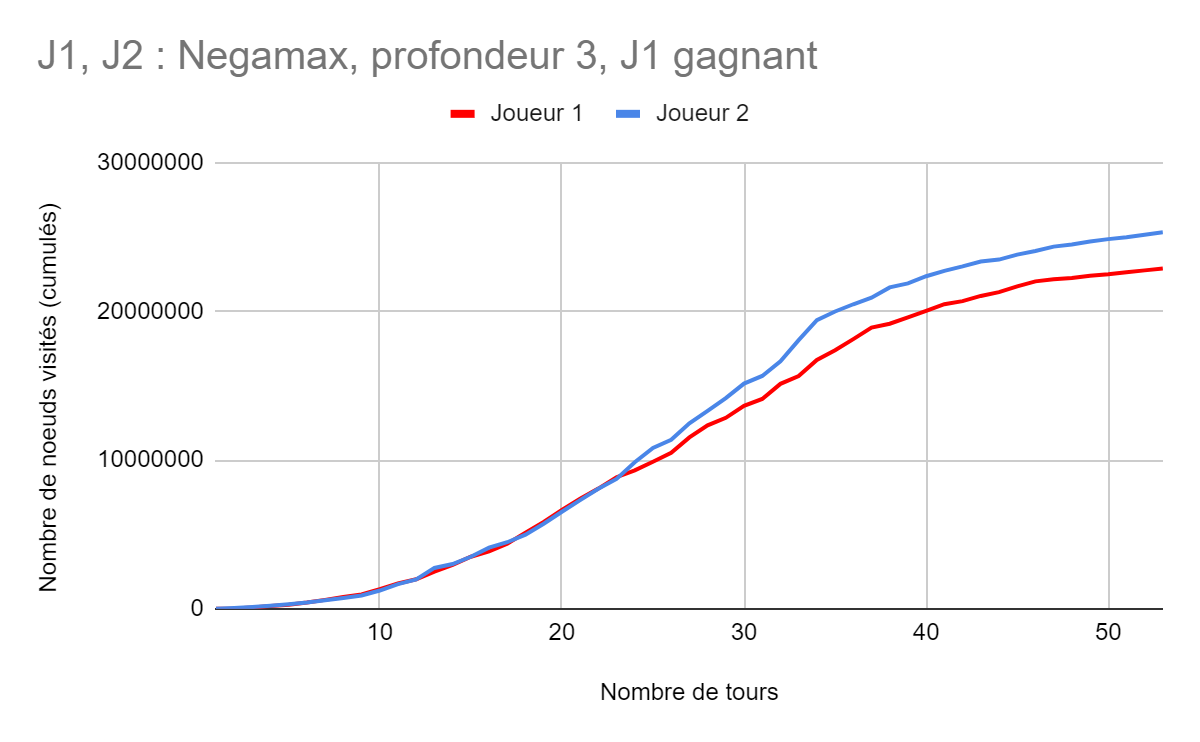
\includegraphics[width=\textwidth]{prof3negamax.png}
\end{figure}

La complexité de cet algorithme est 15 fois supérieur au précédent.\\
Le joueur 2 commence à avoir un avantage au tour 23, avantage qui augmente un peu jusqu’à la fin de la partie. Cependant cet avantage n’est pas suffisant et c’est le premier joueur qui gagne.\\
La courbe est similaire à celles des autres profondeurs.

\newpage
\subsubsection{Profondeur 4}

\begin{figure}[!h]
   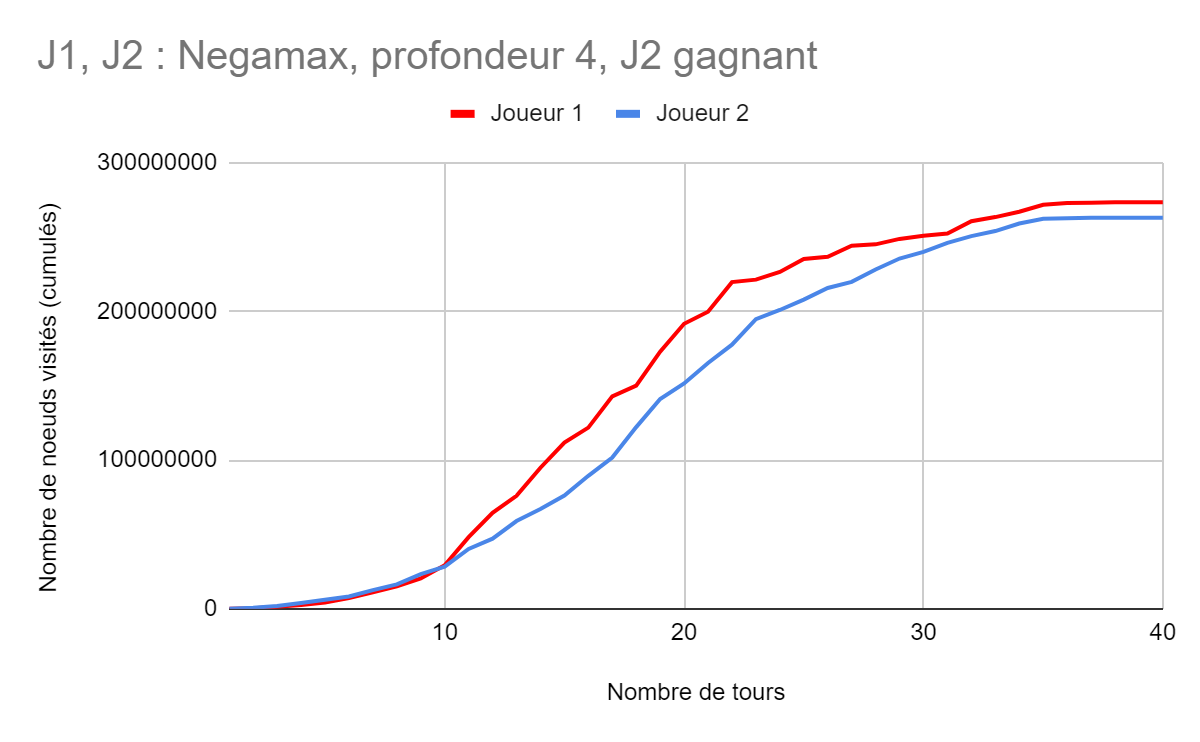
\includegraphics[width=\textwidth]{prof4negamax.png}
\end{figure}

La complexité est environ 11 fois supérieur à Negamax de profondeur 3. Le premier joueur possède un avantage au tour 10 qui augmente jusqu’au tour 22 et se réduit ensuite jusqu’à la fin de la partie.\\
Malgré cet avantage c’est le second joueur qui remporte la partie.

\begin{figure}[!h]
   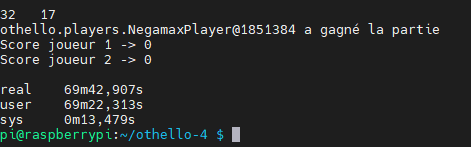
\includegraphics[width=\textwidth]{prof4negamax-console.png}
\end{figure}

Pour le parcours des 536 329 836 nœuds, l’algorithme met 69 minutes et 43 secondes. 

\subsubsection{Profondeur 5}

Nous avons estimé la complexité de Negamax de profondeur 5 à au moins 8.2 milliards de nœuds.\\
Nous avons essayer de le lancer mais après 28 heures d’exécution sur le Raspberry Pi celui-ci n’étais pas terminé, de plus la complexité stocké comme attribut de la classe Player est stocké sur un entier signé 32 bits dont la limite positive est $2^{31} - 1$ soit inférieur à 8 milliards.

\subsubsection{Conclusion de Negamax}

L’augmentation de la complexité en fonction de la profondeur de l’algorithme est exponentielle.\\
La victoire d’un joueur n’a pas l’air influé par son avantage ou par son ordre de jeu.\\
Cet algorithme est très long et du à sa complexité exponentielle, son temps d’exécution l’est également.

\section{Difficultés rencontrés}

Nous avons rencontrés quelques difficultés durant la réalisation du jeu, notamment du à des incompréhension des règles du jeu:\\

\begin{itemize}
    \item Lors du clonage toutes les cases même inoccupées étaient modifiées.
    \item Le saut était possible même quand il n'y avait pas de pion en dessous et ne transformait pas les pions adverses.
\end{itemize}

\section{Expérimentations}

Nous avons mis en place un logger afin de pouvoir exporter plus facilement les données notamment pour faire les graphiques.\\

Le flux s'ouvre au lancement du programme et se ferme à sa fermeture ce qui fait que les fichiers de log resteront vides pendant le fonctionnement du programme, ce qui rend impossible la lecture de la complexité durant le fonctionnement du programme notamment pour le negamax de profondeur 5 ou plus qui demande beaucoup de performances et de temps de calcul.


\section{Conclusion}
\end{document}